\section{light  Class Reference}
\label{classlight}\index{light@{light}}
Simple light point source. 


{\tt \#include $<$light.hpp$>$}

Inheritance diagram for light::\begin{figure}[H]
\begin{center}
\leavevmode
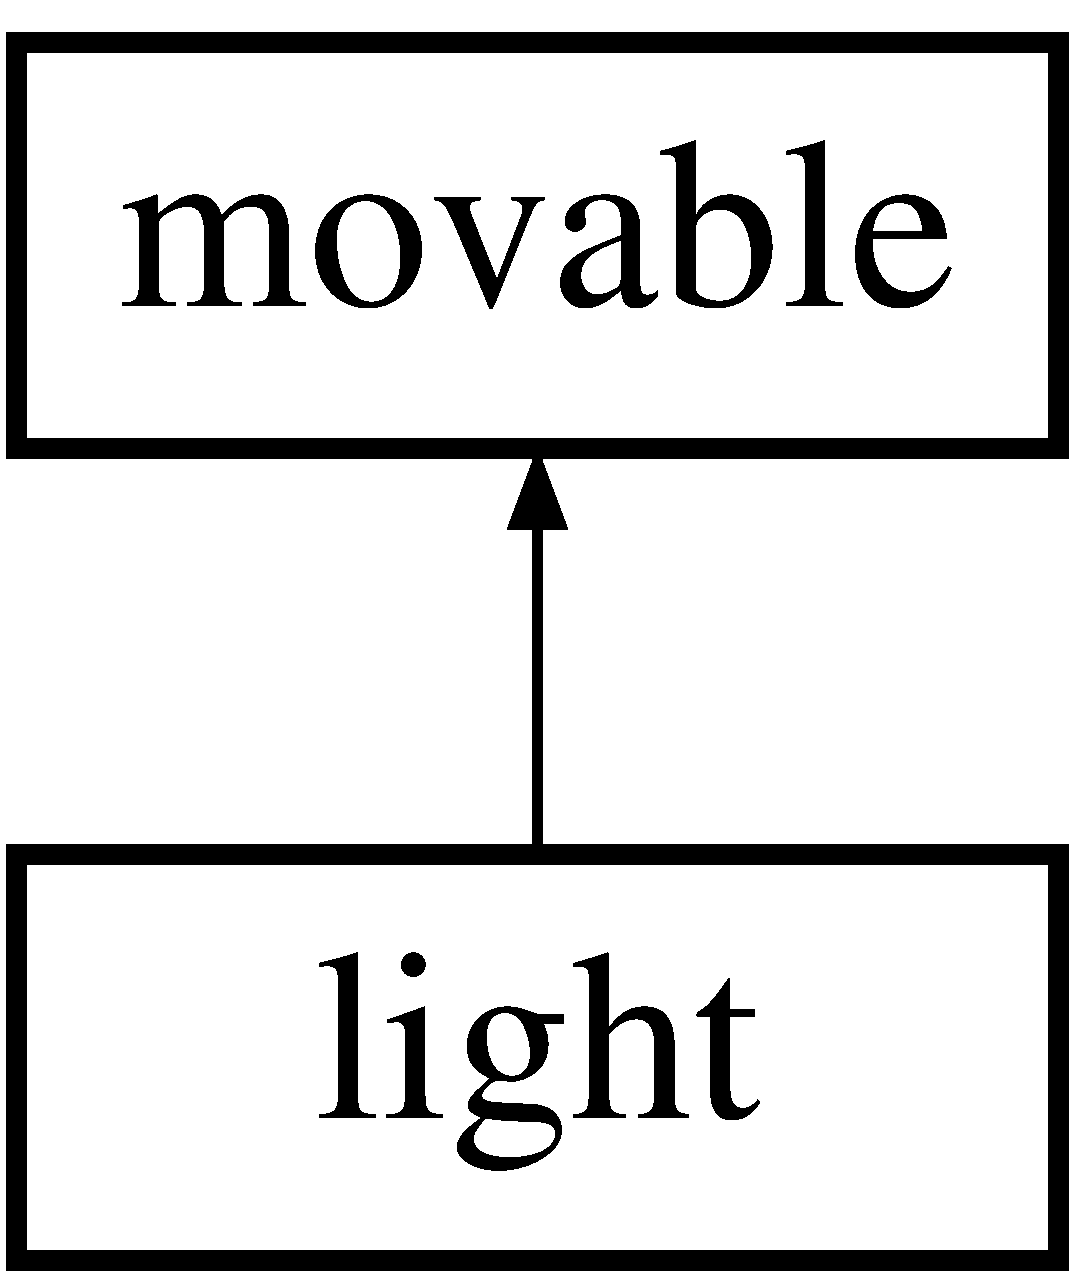
\includegraphics[height=2cm]{classlight}
\end{center}
\end{figure}
\subsection*{Public Methods}
\begin{CompactItemize}
\item 
\index{light@{light}!light@{light}}\index{light@{light}!light@{light}}
{\bf light} ()\label{classlight_a0}

\item 
\index{~light@{$\sim$light}!light@{light}}\index{light@{light}!~light@{$\sim$light}}
{\bf $\sim$light} ()\label{classlight_a1}

\item 
\index{light@{light}!light@{light}}\index{light@{light}!light@{light}}
{\bf light} ({\bf camera} $\ast$viewer, int number, float {\bf max\-Fade}=0, float {\bf min\-Fade}=0, float {\bf scale}=1.0f)\label{classlight_a2}

\item 
\index{draw@{draw}!light@{light}}\index{light@{light}!draw@{draw}}
void {\bf draw} ()\label{classlight_a3}

\item 
\index{drawDim@{drawDim}!light@{light}}\index{light@{light}!drawDim@{draw\-Dim}}
void {\bf draw\-Dim} ({\bf vector3f} distant)\label{classlight_a4}

\item 
\index{update@{update}!light@{light}}\index{light@{light}!update@{update}}
void {\bf update} ()\label{classlight_a5}

\item 
\index{getBoundingBox@{getBoundingBox}!light@{light}}\index{light@{light}!getBoundingBox@{get\-Bounding\-Box}}
void {\bf get\-Bounding\-Box} ()\label{classlight_a6}

\end{CompactItemize}
\subsection*{Public Attributes}
\begin{CompactItemize}
\item 
\index{viewer@{viewer}!light@{light}}\index{light@{light}!viewer@{viewer}}
{\bf camera} $\ast$ {\bf viewer}\label{classlight_m0}

\item 
float {\bf max\-Fade}
\begin{CompactList}\small\item\em Distance at which the light is completely dim.\item\end{CompactList}\item 
\index{minFade@{minFade}!light@{light}}\index{light@{light}!minFade@{min\-Fade}}
float {\bf min\-Fade}\label{classlight_m2}

\begin{CompactList}\small\item\em Minimum istance at which the light maximally bright.\item\end{CompactList}\item 
\index{scale@{scale}!light@{light}}\index{light@{light}!scale@{scale}}
float {\bf scale}\label{classlight_m3}

\begin{CompactList}\small\item\em How to scale the brightness- $>$1.0 will be clamped, so bright lights will wash out.\item\end{CompactList}\item 
GLfloat {\bf Ka} [4]
\item 
\index{Kd@{Kd}!light@{light}}\index{light@{light}!Kd@{Kd}}
GLfloat {\bf Kd} [4]\label{classlight_m5}

\item 
\index{Ks@{Ks}!light@{light}}\index{light@{light}!Ks@{Ks}}
GLfloat {\bf Ks} [4]\label{classlight_m6}

\item 
\index{GL_LIGHTX@{GL\_\-LIGHTX}!light@{light}}\index{light@{light}!GL_LIGHTX@{GL\_\-LIGHTX}}
int {\bf GL\_\-LIGHTX}\label{classlight_m7}

\begin{CompactList}\small\item\em From 0-7 (or how ever many lights can be handled at once).\item\end{CompactList}\item 
\index{verbose@{verbose}!light@{light}}\index{light@{light}!verbose@{verbose}}
bool {\bf verbose}\label{classlight_m8}

\begin{CompactList}\small\item\em Stdout toggle.\item\end{CompactList}\end{CompactItemize}


\subsection{Detailed Description}
Simple light point source.

So far just hold the light color parameters and the location.

Orientation is also stored even though a rotated point source is indistuinguishable from the non-rotated.

There's also a visible .obj shell around the light in order to  make placement possible (rather than guessing the lights position by looking at it's effect on normal objects).

There's no diminishment with distance, that would be interesting to implement and though I can think of at least one way to do it  (objects would be individually lit with a distance scaling factor, and perhaps the distance to the light would also have the object be split up for lighting in order to show a differential across it's surface), I'm curious what the conventional way is. 



\subsection{Member Data Documentation}
\index{light@{light}!Ka@{Ka}}
\index{Ka@{Ka}!light@{light}}
\subsubsection{\setlength{\rightskip}{0pt plus 5cm}GLfloat light::Ka[4]}\label{classlight_m4}


Currently lights aren't directional, so only keep a vector of position and orientation doesn't matter. {\bf vector3f} {\rm (p.\,\pageref{classvector3f})} $\ast$position; \index{light@{light}!maxFade@{maxFade}}
\index{maxFade@{maxFade}!light@{light}}
\subsubsection{\setlength{\rightskip}{0pt plus 5cm}float light::max\-Fade}\label{classlight_m1}


Distance at which the light is completely dim.

max\-Fade = 0 means no linear scaling -$>$ uniform at any difference 

The documentation for this class was generated from the following files:\begin{CompactItemize}
\item 
{\bf light.hpp}\item 
light.cpp\end{CompactItemize}
